\documentclass[10pt,twocolumn]{article}

% Packages
\usepackage[margin=0.75in]{geometry}
\usepackage{algorithm}
\usepackage{algorithmic}
\usepackage{booktabs}
\usepackage{amsmath,amssymb}
\usepackage{multirow}
\usepackage{graphicx}
\usepackage{hyperref}
\usepackage{enumitem}
\setlist{nosep,leftmargin=*}
\usepackage{tikz}
\usetikzlibrary{positioning, arrows.meta, fit, backgrounds, calc}

% Figure colors
\definecolor{rescolor}{RGB}{215, 130, 42}
\definecolor{pipcolor}{RGB}{65, 130, 200}
\definecolor{ilcolor}{RGB}{120, 95, 220}
\definecolor{metcolor}{RGB}{40, 128, 80}
\definecolor{deccolor}{RGB}{190, 80, 80}
\definecolor{frzcolor}{RGB}{120, 120, 120}

\pagestyle{plain}

% Notation shortcuts
\newcommand{\cR}{\mathcal{R}}
\newcommand{\cM}{\mathcal{M}}
\newcommand{\cG}{\mathcal{G}}
\newcommand{\cC}{\mathcal{C}}
\newcommand{\bm}{\mathbf{m}}

\begin{document}

\title{Automated Research for LLM Policy Synthesis\\in Sequential Social Dilemmas}

\author{V\'ictor Gallego\\
\small Komorebi AI Technologies, Madrid, Spain\\
\small \texttt{victor.gallego@komorebi.ai}}
\date{}

\maketitle

\begin{abstract}
We apply the \emph{autoresearch} paradigm to multi-agent LLM policy synthesis. A \emph{researcher agent} $\cR$ (Claude Opus 4.6) iteratively modifies the synthesis pipeline---system prompts, feedback construction, helper libraries, iteration logic---under which a \emph{policy-synthesizer} LLM $\cM$ generates cooperative strategies for Sequential Social Dilemmas. The researcher never modifies the environment or evaluation; everything else is fair game. We conduct 12 autonomous runs across two games (Cleanup and Gathering), two policy LLMs (Gemini 3.1 Pro and Claude Sonnet 4.6), and two social welfare objectives (utilitarian efficiency and Rawlsian maximin). The researcher reliably exceeds hand-designed baselines: in Cleanup, efficiency improves by 16\% (Gemini) and 128\% (Sonnet) over the dense feedback configuration of prior work. Most strikingly, maximin-optimized pipelines achieve near-perfect equality ($E{=}0.98$) with negligible efficiency loss ($-1\%$), discovering duty rotation as the key fairness mechanism---never found under efficiency optimization. The contrast with Gathering, where efficiency optimization alone yields $E{>}0.94$, reveals that game structure determines whether fairness requires explicit optimization: in provision dilemmas fairness needs designed mechanisms, while in restraint dilemmas it emerges as a byproduct of coordination.
\end{abstract}

%% ============================================================
\section{Background}
%% ============================================================

We build on the iterative LLM policy synthesis framework of Gallego~\cite{gallego2026}. An SSD is a partially observable Markov game $\cG = \langle N, \mathcal{S}, \{A_i\}_{i=1}^{N}, T, \{R_i\}_{i=1}^{N}, H \rangle$. Social outcomes are evaluated via four metrics~\cite{perolat2017}: efficiency $U$, equality $E$, sustainability $S$, and peace $P$. We additionally consider the \emph{maximin} (Rawlsian) welfare criterion $\min_i R_i$, which maximizes the return of the worst-off agent.

We study two SSDs that represent complementary dilemma types. \textbf{Cleanup}~\cite{hughes2018} is a \emph{public goods provision} game ($N{=}10$): a river accumulates waste while an orchard grows apples. Cleaning costs $-1$ per beam but enables apple regrowth for everyone ($+1$ per apple). The dilemma: free-ride on cleaning vs.\ contribute. \textbf{Gathering}~\cite{leibo2017,perolat2017} is a \emph{common pool resource} game ($N{=}4$): agents collect shared apples and may tag rivals to temporarily remove them. The dilemma: over-harvest and aggress vs.\ cooperate and share. The games differ in their cost structure---asymmetric provision vs.\ symmetric restraint---a distinction that drives our key findings.

A frozen LLM $\cM$ acts as a policy synthesizer. Given a system prompt $p$ and a feedback prompt $q_k$, it generates a Python policy $\pi_{k+1} = \cM(p, q(\pi_k, \mathcal{F}_k^\ell))$, where $\ell$ specifies the feedback level and $\mathcal{F}_k = (\bar{r}_k, \bm_k)$ contains the mean per-agent reward $\bar{r}_k$ and the social metrics vector $\bm_k = (U_k, E_k, S_k, P_k)$. All $N$ agents execute the same policy (homogeneous self-play). Gallego~\cite{gallego2026} compared two hand-designed feedback levels---sparse (reward-only) and dense (reward + social metrics)---and showed that dense feedback consistently improves cooperative outcomes. The dense feedback configuration achieves $U{=}1.93{\pm}0.73$ (Gemini) and $U{=}0.86{\pm}0.62$ (Sonnet) on Cleanup.

%% ============================================================
\section{Two-Level Framework}
%% ============================================================

We introduce a two-level system where a \emph{researcher agent} $\cR$ optimizes the conditions under which the policy synthesizer $\cM$ operates. The key insight is that the entire inner-loop codebase---not just the feedback level---is a designable artifact. Figure~\ref{fig:framework} illustrates the architecture.

\begin{figure}[t]
\centering
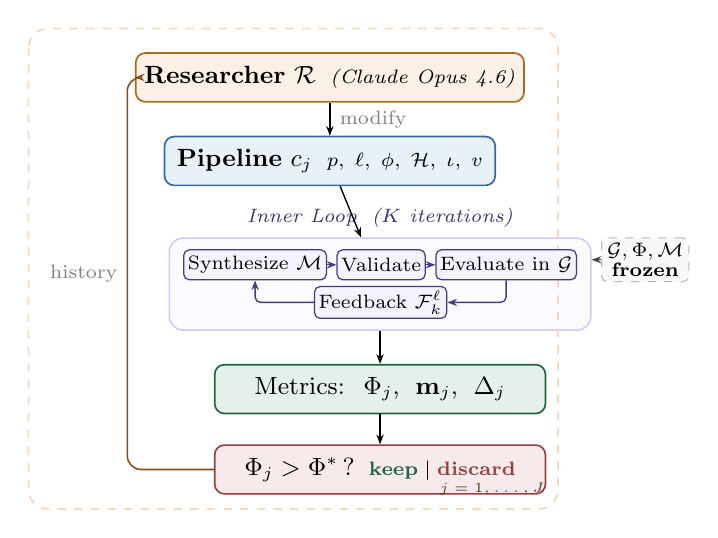
\begin{tikzpicture}[
  >={Stealth[length=3.5pt]},
  node distance=0.4cm,
  % --- Styles ---
  mbox/.style={
    rectangle, rounded corners=3.5pt, draw=#1!80!black, fill=#1!12,
    line width=0.6pt, minimum height=0.62cm, minimum width=4.2cm,
    align=center, inner sep=3pt, font=\small},
  sbox/.style={
    rectangle, rounded corners=2pt, draw=ilcolor!60!black, fill=ilcolor!8,
    line width=0.45pt, minimum height=0.38cm,
    align=center, inner sep=1.5pt, font=\scriptsize},
  frzbox/.style={
    rectangle, rounded corners=2pt, draw=frzcolor!55, fill=frzcolor!5,
    dashed, line width=0.4pt, align=center, inner sep=2pt, font=\scriptsize},
  myarr/.style={->, line width=0.5pt, #1!60!black},
  myarr/.default=black,
  albl/.style={font=\scriptsize, text=black!50},
]
% === NODES ===
% 1. Researcher
\node[mbox=rescolor] (R) {%
  \textbf{Researcher} $\cR$%
  \;\;{\scriptsize\textit{(Claude Opus 4.6)}}};
% 2. Pipeline
\node[mbox=pipcolor, below=0.42cm of R] (P) {%
  \textbf{Pipeline} $c_j$%
  \;\;{\scriptsize $p,\;\ell,\;\phi,\;\mathcal{H},\;\iota,\;v$}};
% 3. Inner loop sub-nodes
\node[sbox, below=0.8cm of P, xshift=-0.95cm] (S) {Synthesize $\cM$};
\node[sbox, right=0.12cm of S] (V) {Validate};
\node[sbox, right=0.12cm of V] (Ev) {Evaluate in $\cG$};
% Feedback below
\coordinate (fbmid) at ($(S.south)!0.5!(Ev.south)+(0,-0.28)$);
\node[sbox, minimum width=0.9cm] at (fbmid) (FB) {Feedback $\mathcal{F}_k^\ell$};
% Inner loop frame
\begin{scope}[on background layer]
\node[draw=ilcolor!35, fill=ilcolor!3, rounded corners=5pt, line width=0.55pt,
      inner xsep=5pt, inner ysep=4pt,
      fit=(S)(V)(Ev)(FB),
      label={[font=\scriptsize\itshape, text=ilcolor!50!black]%
             above:{Inner Loop \;($K$ iterations)}}
      ] (IL) {};
\end{scope}
% 4. Metrics
\node[mbox=metcolor, below=0.42cm of IL] (M) {%
  Metrics:\; $\Phi_j$,\; $\mathbf{m}_j$,\; $\Delta_j$};
% 5. Decision
\node[mbox=deccolor, below=0.38cm of M] (D) {%
  $\Phi_j > \Phi^*$\,?\;\;%
  {\scriptsize\textcolor{metcolor!80!black}{\textbf{keep}}%
   \;$\mid$\;%
   \textcolor{deccolor!80!black}{\textbf{discard}}}};
% Frozen annotation
\node[frzbox, right=0.12cm of IL.north east, anchor=north west] (F) {%
  $\cG$,\,$\Phi$,\,$\cM$\\[-1pt]\textbf{frozen}};

% === ARROWS ===
% Main vertical flow
\draw[myarr] (R) -- node[albl, right] {modify} (P);
\draw[myarr] (P) -- (IL);
\draw[myarr] (IL) -- (M);
\draw[myarr] (M) -- (D);
% Inner cycle
\draw[myarr=ilcolor] (S) -- (V);
\draw[myarr=ilcolor] (V) -- (Ev);
\draw[myarr=ilcolor, rounded corners=2pt] (Ev.south) |- (FB);
\draw[myarr=ilcolor, rounded corners=2pt] (FB) -| (S.south);
% Frozen pointer
\draw[myarr=frzcolor, dashed] (F.west) -- (IL.east |- F.west);
% Outer loop feedback
\draw[myarr=rescolor, rounded corners=5pt, line width=0.55pt]
  (D.west) -- ++(-1.1,0) |-
  node[albl, left, pos=0.25] {history} (R.west);

% === OUTER FRAME ===
\begin{scope}[on background layer]
\draw[rescolor!30, dashed, rounded corners=7pt, line width=0.65pt]
  ([shift={(-1.35cm,0.3cm)}]R.north west) rectangle
  ([shift={(0.15cm,-0.18cm)}]D.south east);
\end{scope}
\node[font=\tiny\itshape, text=rescolor!45!black, anchor=south east]
  at ([shift={(0.1cm,-0.13cm)}]D.south east) {$j = 1,\ldots,J$};
\end{tikzpicture}
\caption{Two-level automated research framework (Algorithm~\ref{alg:outer}). \emph{Outer loop}: the researcher $\cR$ modifies the pipeline configuration $c_j$, runs the inner loop, and keeps or discards based on $\Phi$. \emph{Inner loop}: the policy LLM $\cM$ iteratively synthesizes, validates, and evaluates policies in the frozen environment $\cG$.}
\label{fig:framework}
\end{figure}

\subsection{Configuration Space}

Let $\cC$ denote the space of \emph{pipeline configurations}. Each configuration $c \in \cC$ specifies the full inner-loop setup:
\begin{equation}
  c = (p,\, \ell,\, \phi,\, \mathcal{H},\, \iota,\, v)
\end{equation}
where $p$ is the system prompt, $\ell$ is the feedback template, $\phi$ is the feedback construction function, $\mathcal{H}$ is the helper function library, $\iota$ specifies the iteration logic (number of iterations $K$, sampling strategy, temperature schedule), and $v$ is the validation pipeline. Table~\ref{tab:config} provides concrete examples.

\begin{table}[t]
\caption{Configuration components modifiable by the researcher. The environment simulator, ground-truth evaluation, and policy LLM weights are frozen.}
\label{tab:config}
\centering
\small
\begin{tabular}{@{}lll@{}}
\toprule
 & Scope & Examples \\
\midrule
$p$ & System prompt & Hints, worked examples \\
$\ell$ & Feedback template & Metric subset, framing \\
$\phi$ & Feedback fn & Derived metrics, trends \\
$\mathcal{H}$ & Helper library & Pathfinding, zones \\
$\iota$ & Iteration logic & $K$, eval seeds, best-of-$n$ \\
$v$ & Validation & Safety checks, smoke tests \\
\bottomrule
\end{tabular}
\end{table}

The sparse vs.\ dense comparison of~\cite{gallego2026} corresponds to a single binary choice within the $\ell$ component. Our framework opens the full configuration space to automated search.

\subsection{Inner Loop (Policy Synthesis)}

Given a configuration $c$, the inner loop executes $K$ iterations of LLM policy synthesis:
\begin{equation}
  \pi^*_c = \textsc{InnerLoop}(\cM, \cG, c)
\end{equation}
following Algorithm~1 of~\cite{gallego2026}: at each iteration $k$, $\cM$ generates a policy from the system prompt $p$ and feedback constructed according to $(\ell, \phi)$, using helpers $\mathcal{H}$. The policy is validated via $v$ and evaluated in $N$-agent self-play over seeds $S$.

The inner loop output is evaluated on held-out seeds via a fixed ground-truth objective:
\begin{equation}
  \Phi(c) = \textsc{Eval}(\pi^*_c;\; \cG,\; S_{\text{held-out}})
  \label{eq:phi}
\end{equation}
where $\Phi$ maps from social outcomes to a scalar. We consider two objectives:
\begin{align}
  \Phi_U &= U & \text{(utilitarian efficiency)} \label{eq:eff}\\
  \Phi_{\min} &= \min_i R_i & \text{(Rawlsian maximin)} \label{eq:rawls}
\end{align}

\subsection{Outer Loop (Automated Research)}

The researcher agent $\cR$ iteratively modifies the pipeline configuration. Following the autoresearch paradigm~\cite{karpathy2026}, $\cR$ operates on the inner-loop codebase as a modifiable artifact, proposing changes, observing outcomes, and refining. The procedure is formalized in Algorithm~\ref{alg:outer}.

\begin{algorithm}[t]
\caption{Two-Level Automated Research}
\label{alg:outer}
\begin{algorithmic}[1]
\REQUIRE Game $\cG$, policy synthesizer $\cM$, researcher $\cR$, system prompt for researcher $p_\cR$, initial configuration $c_0$, outer iterations $J$, ground-truth objective $\Phi$, held-out seeds $S_{\text{held-out}}$
\ENSURE Best configuration $c^*$, best policy $\pi^*$
\STATE $\pi^*_0 \leftarrow \textsc{InnerLoop}(\cM, \cG, c_0)$
\STATE $\Phi_0 \leftarrow \textsc{Eval}(\pi^*_0;\; \cG,\; S_{\text{held-out}})$
\STATE $\textit{history} \leftarrow \{(c_0, \Phi_0, \bm_0, \varnothing)\}$
\FOR{$j = 1, \dots, J$}
  \STATE $c_j \leftarrow \cR\!\left(p_\cR,\; \textsc{code}(c_{j-1}),\; \textit{history}\right)$
  \STATE \textbf{if} $\neg\,\textsc{ValidateConfig}(c_j)$ \textbf{then} retry $\leq R$ times
  \STATE $\pi^*_j \leftarrow \textsc{InnerLoop}(\cM, \cG, c_j)$
  \STATE $\Phi_j \leftarrow \textsc{Eval}(\pi^*_j;\; \cG,\; S_{\text{held-out}})$
  \STATE $\Delta_j \leftarrow \textsc{Diff}(c_{j-1}, c_j)$ \hfill \textit{// code diff}
  \STATE $\textit{history} \leftarrow \textit{history} \cup \{(c_j, \Phi_j, \bm_j, \Delta_j)\}$
\ENDFOR
\STATE $j^* \leftarrow \arg\max_j \Phi_j$
\RETURN $c_{j^*},\; \pi^*_{j^*}$
\end{algorithmic}
\end{algorithm}

At each outer iteration $j$, the researcher $\cR$ receives:
\begin{itemize}
  \item The \textbf{full source code} of the current configuration $c_{j-1}$ (prompts, feedback construction, helpers, iteration logic).
  \item The \textbf{experiment history}: for each prior iteration, the code diff $\Delta_i$, ground-truth score $\Phi_i$, and social metrics vector $\bm_i$.
  \item The \textbf{environment source code} (read-only), enabling the researcher to reason about game mechanics.
\end{itemize}

The researcher proposes a new configuration $c_j$ by generating code modifications. This mirrors the autoresearch setup, where an AI agent modifies \texttt{train.py} and observes validation loss; here, the researcher modifies the inner-loop codebase and observes social welfare.

\subsection{Structural Analogy}

Table~\ref{tab:analogy} formalizes the correspondence between autoresearch for LLM pretraining and our two-level system.

\begin{table}[t]
\caption{Structural analogy between autoresearch~\cite{karpathy2026} for LLM pretraining and our framework for multi-agent policy synthesis.}
\label{tab:analogy}
\centering
\small
\begin{tabular}{@{}lll@{}}
\toprule
 & Autoresearch & This work \\
\midrule
Modifiable & \texttt{train.py} & Inner-loop codebase \\
artifact & (model + optimizer) & $(p, \ell, \phi, \mathcal{H}, \iota, v)$ \\
\addlinespace
Frozen & \texttt{prepare.py} & Environment $\cG$, \\
infrastructure & (data, tokenizer, eval) & eval $\Phi$, LLM $\cM$ \\
\addlinespace
Metric & val\_bpb $\downarrow$ & $\Phi$ (social welfare) $\uparrow$ \\
\addlinespace
Budget & 5 min wall clock & $K$ iters $\times$ $|S|$ seeds \\
\addlinespace
Agent & AI coding agent & Researcher $\cR$ \\
\bottomrule
\end{tabular}
\end{table}

The key structural property shared by both systems: the agent modifies \emph{how learning happens} (the pipeline/training code), not the learned artifact directly (the policy/model weights). The output of each outer iteration is a \emph{reusable configuration}---transferable across policy LLMs, games, and random seeds---rather than a single policy.

\subsection{Design Principles}

\paragraph{Separation of concerns.}
The researcher $\cR$ and the synthesizer $\cM$ are distinct LLM calls with distinct roles. $\cR$ reasons about \emph{what information and tools help $\cM$ write better policies}; $\cM$ reasons about \emph{what policy to write given its current context}. Using different underlying models ($\cR \neq \cM$) avoids conflation and enables cross-model experiments.

\paragraph{Read-only environment.}
The researcher can read the environment source code to understand game mechanics but cannot modify the simulator. This prevents the trivial solution of making the game easier and cleanly separates mechanism design from environment design.

\paragraph{Fixed compute budget.}
Each inner loop runs for exactly $K$ iterations with $|S|$ seeds. The researcher cannot inflate performance by running more iterations, but can change what happens \emph{within} those $K$ iterations (e.g., best-of-$n$ sampling, varying the prompt structure mid-run).

\paragraph{Diff-based history.}
The researcher sees code diffs $\Delta_j$ from previous experiments alongside their outcomes. This enables causal reasoning about which modifications drove which improvements, mirroring autoresearch's experiment logs.

%% ============================================================
\section{Connection to Automated Mechanism Design}
%% ============================================================

The two-level structure admits a mechanism design interpretation. The researcher $\cR$ acts as a \emph{mechanism designer}: it controls the information structure (what metrics to reveal, how to frame them), the action space (what helper functions are available), and the incentive structure (how feedback is presented) under which the policy synthesizer $\cM$ operates. The synthesizer acts as the \emph{agent} within the designed mechanism.

This connects to the automated mechanism design literature~\cite{conitzer2002}, where a principal designs rules to induce desired behavior from self-interested agents. In our setting:
\begin{itemize}
  \item The \textbf{principal} is the researcher $\cR$, optimizing the ground-truth objective $\Phi$.
  \item The \textbf{agent} is the synthesizer $\cM$, optimizing per-agent reward as instructed.
  \item The \textbf{mechanism} is the configuration $c$: prompts, feedback, helpers, iteration logic.
  \item The \textbf{outcome} is the social welfare of the resulting multi-agent policy $\pi^*_c$.
\end{itemize}

A key distinction from classical mechanism design: $\cM$ is not \emph{strategically} self-interested---it follows instructions---but it has \emph{bounded rationality} in the sense that its ability to synthesize effective policies depends on the information and tools provided. The researcher's task is thus closer to \emph{information design}~\cite{kamenica2011}: choosing what to reveal to help $\cM$ navigate the cooperation--defection tension. Our experiments (Section~\ref{sec:experiments}) show that the researcher designs qualitatively different information structures depending on the welfare objective $\Phi$, supporting this interpretation empirically.

%% ============================================================
\section{Experiments}
\label{sec:experiments}
%% ============================================================

\subsection{Setup}

We conduct 12 autonomous researcher runs across a factorial design. The researcher agent $\cR$ is Claude Opus 4.6 in all runs. Each run operates on a dedicated git branch, modifying only the pipeline files (\texttt{pipeline/}).

\paragraph{Design.}
For Cleanup: $2$ policy LLMs $\times$ $2$ objectives $\times$ $2$ replications $=$ 8 runs. For Gathering: $2$ policy LLMs $\times$ $1$ objective $\times$ $2$ replications $=$ 4 runs. Maximin runs are unnecessary for Gathering because efficiency optimization alone achieves equality $E > 0.94$ (the game's symmetric cost structure makes fairness a free byproduct of coordination).

\paragraph{Models.}
Policy synthesizer $\cM$: Gemini 3.1 Pro (Google) or Claude Sonnet 4.6 (Anthropic). Both use extended thinking. These are the same models evaluated in~\cite{gallego2026}.

\paragraph{Baselines.}
The hand-designed dense feedback (reward + social metrics) configuration from~\cite{gallego2026} serves as the initial pipeline $c_0$ for all runs. On Cleanup ($N{=}10$), this baseline achieves $U{=}1.93{\pm}0.73$ with Gemini and $U{=}0.86{\pm}0.62$ with Sonnet (mean $\pm$ s.d.\ across 4 runs each).

\paragraph{Inner loop parameters.}
$K{=}3$ synthesis iterations (or $K{=}2$ if the researcher elects), evaluated over $|S|{=}5$--$12$ random seeds (researcher-configurable). The researcher ran $J{=}3$--$17$ outer iterations per run (mean: 8.3), with a keep rate of 18\%--100\% (mean: 63\%).

\subsection{Results}

Table~\ref{tab:results} presents the main results, showing the best configuration achieved by the researcher in each condition, compared against the hand-designed baseline of~\cite{gallego2026}.

\begin{table}[t]
\caption{Autoresearch results. Mean $\pm$ s.d.\ across runs per condition (2 runs for autoresearch, 4 for Cleanup baselines, 2 for Gathering baselines). Baseline: unmodified pipeline with dense feedback from~\cite{gallego2026}.}
\label{tab:results}
\centering
\small
\begin{tabular}{@{}llccc@{}}
\toprule
Policy LLM & Target & $U$ & $E$ & $\min_i R_i$ \\
\midrule
\multicolumn{5}{@{}l}{\emph{Cleanup ($N{=}10$) --- Baseline}} \\
Gemini 3.1 Pro & --- & 1.93{\scriptsize$\pm$0.73} & 0.17{\scriptsize$\pm$0.52} & --- \\
Sonnet 4.6 & --- & 0.86{\scriptsize$\pm$0.62} & $-$0.02{\scriptsize$\pm$0.36} & --- \\
\addlinespace
\multicolumn{5}{@{}l}{\emph{Cleanup ($N{=}10$) --- Autoresearch}} \\
\multirow{2}{*}{Gemini 3.1 Pro}
  & $\Phi_U$ & \textbf{3.20}{\scriptsize$\pm$0.05} & 0.55{\scriptsize$\pm$0.06} & --- \\
  & $\Phi_{\min}$ & 3.16{\scriptsize$\pm$0.04} & \textbf{0.98}{\scriptsize$\pm$0.00} & \textbf{290}{\scriptsize$\pm$6} \\
\addlinespace
\multirow{2}{*}{Sonnet 4.6}
  & $\Phi_U$ & \textbf{3.12}{\scriptsize$\pm$0.02} & 0.66{\scriptsize$\pm$0.03} & --- \\
  & $\Phi_{\min}$ & 2.57{\scriptsize$\pm$0.36} & \textbf{0.91}{\scriptsize$\pm$0.07} & \textbf{179}{\scriptsize$\pm$20} \\
\midrule
\multicolumn{5}{@{}l}{\emph{Gathering ($N{=}4$) --- Baseline}} \\
Gemini 3.1 Pro & --- & 2.04{\scriptsize$\pm$0.54} & 0.90{\scriptsize$\pm$0.11} & 412{\scriptsize$\pm$224} \\
Sonnet 4.6 & --- & 0.03{\scriptsize$\pm$0.00} & 0.54{\scriptsize$\pm$0.00} & 0{\scriptsize$\pm$0} \\
\addlinespace
\multicolumn{5}{@{}l}{\emph{Gathering ($N{=}4$) --- Autoresearch}} \\
Gemini 3.1 Pro & $\Phi_U$ & 2.49{\scriptsize$\pm$0.02} & 0.98{\scriptsize$\pm$0.00} & 582{\scriptsize$\pm$1} \\
Sonnet 4.6 & $\Phi_U$ & 2.52{\scriptsize$\pm$0.01} & 0.96{\scriptsize$\pm$0.02} & 576{\scriptsize$\pm$20} \\
\bottomrule
\end{tabular}
\end{table}

\paragraph{Finding 1: The researcher reliably improves over hand-designed baselines.}
All 12 runs show substantial improvement regardless of starting point (Figure~\ref{fig:efficiency}). In Cleanup, the researcher exceeds the unmodified pipeline baseline by 66\% with Gemini ($U$: $1.93 \to 3.20$) and 263\% with Sonnet ($U$: $0.86 \to 3.12$). Strikingly, the Sonnet improvement nearly closes the gap with Gemini ($U{=}3.12$ vs.\ $3.20$), despite a $2\times$ baseline disadvantage ($0.86$ vs.\ $1.93$). Final efficiency values cluster tightly around $U \approx 3.1$--$3.2$ despite baselines varying from $0.29$ to $2.70$ across individual runs, suggesting the researcher reliably discovers the performance ceiling of each policy LLM. Beyond improving the mean, the researcher also dramatically reduces variance: in Cleanup, Gemini's s.d.\ drops from $0.73$ to $0.05$ ($14\times$ reduction) and Sonnet's from $0.62$ to $0.02$ ($31\times$) under efficiency optimization. In Gathering, Gemini's s.d.\ drops from $0.54$ to $0.02$. The researcher discovers pipeline modifications---structured helpers, strategic hints, tailored feedback---that constrain the policy LLM toward consistently good solutions, reducing dependence on inner-loop stochasticity.

\begin{figure*}[t]
\centering
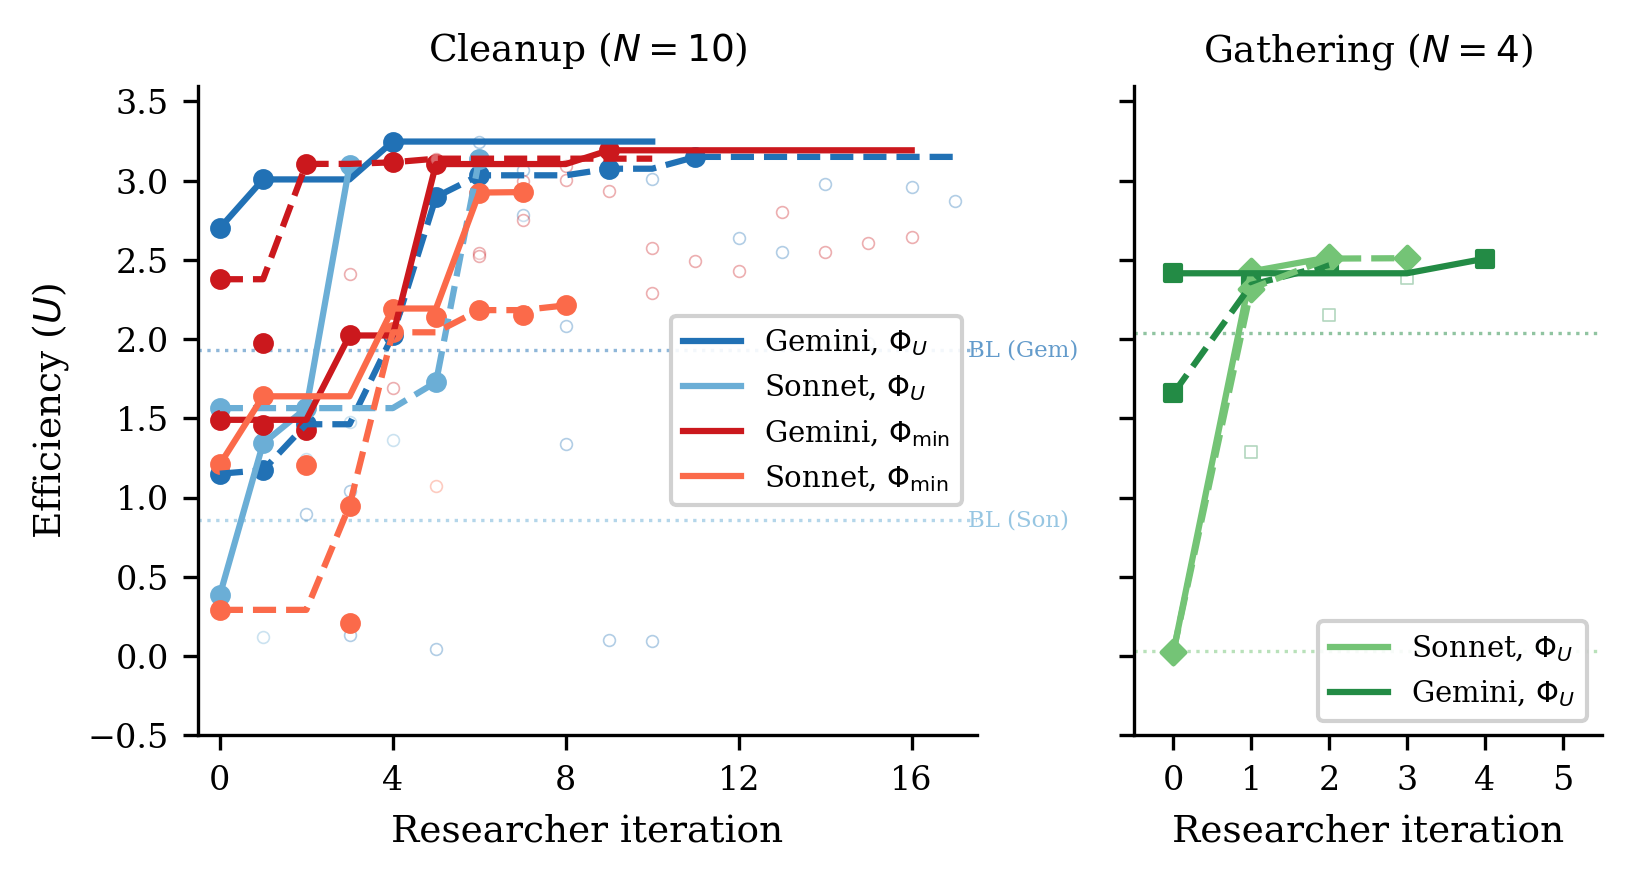
\includegraphics[width=0.95\textwidth]{autoresearch/figures/fig1_efficiency_trajectory.png}
\caption{Efficiency ($U$) across researcher iterations for all 12 runs. \emph{Left}: Cleanup ($N{=}10$) with 8 runs across 2 LLMs $\times$ 2 objectives (solid lines = kept experiments, open circles = discarded). Dashed horizontal line: hand-designed baseline from~\cite{gallego2026}. All runs converge to $U \approx 3.1$--$3.2$ despite diverse starting points. \emph{Right}: Gathering ($N{=}4$) with 4 runs (2 per LLM). All converge to $U \approx 2.5$ within 2--4 iterations despite baselines ranging from $0.03$ to $2.42$.}
\label{fig:efficiency}
\end{figure*}

\paragraph{Finding 2: No efficiency--fairness tradeoff in Cleanup (Gemini).}
Maximin-optimized Gemini pipelines sacrifice only $1\%$ efficiency ($U$: $3.16$ vs.\ $3.20$) while achieving near-perfect equality ($E$: $0.98$ vs.\ $0.55$) and transforming maximin from deeply negative baselines ($-99$ to $-84$) to $\min_i R_i = 290$. The researcher discovers that \emph{fair duty rotation}---time-based cycling of cleaning responsibilities using \texttt{agent\_id} and \texttt{env.\_step\_count}---simultaneously improves worst-off welfare \emph{and} collective output. Because cleaning is a public good, distributing the cleaning cost fairly ensures enough cleaners to sustain apple production.

For Sonnet, there is a moderate tradeoff: efficiency drops from $3.12$ to $2.57$ under maximin optimization. The gap reflects Sonnet's harder time implementing complex coordination mechanisms (role rotation, zone assignment) from strategic hints alone.

\paragraph{Finding 3: Game structure determines whether fairness requires explicit optimization.}
In Cleanup, where cleaning costs are borne asymmetrically (cleaners pay $-1$, free-riders collect apples), baseline equality ranges from $E{=}0.04$ to $0.62$, and maximin optimization is required to reach $E > 0.9$. In Gathering, where all agents face a symmetric landscape, efficiency optimization alone achieves $E > 0.94$ across all 4 runs---no separate maximin runs are needed.

This generalizes: in \emph{provision} dilemmas with asymmetric costs, fairness requires designed mechanisms (role rotation, duty sharing); in \emph{restraint} dilemmas with symmetric costs, fairness emerges as a free byproduct of efficient coordination. The researcher independently discovers this---it creates role differentiation pipelines only for Cleanup, and pure spatial-coordination pipelines for Gathering.

\paragraph{Finding 4: Convergent discovery of qualitatively different strategies per objective.}
Despite fully independent runs, the researcher converges on the same core strategies within each condition (Table~\ref{tab:strategies}). In Cleanup, waste-counting helpers and spatial zone partitioning appear across all 8 runs. The key qualitative difference: \emph{role rotation}---time-based cycling of cleaning duty---appears in 4/4 maximin runs but 0/4 efficiency runs. Under efficiency optimization, the researcher assigns static cleaning roles (some agents always clean), achieving high collective output at the cost of equality. Under maximin optimization, it discovers rotation as a fairness mechanism.

In Gathering, the researcher discovers BFS-based Voronoi territory partitioning and respawn-timer awareness, with no role differentiation needed---the entire optimization is spatial (who collects which apples) and temporal (respawn-aware positioning).

\begin{table}[t]
\caption{Strategies discovered by the researcher in Cleanup across 4 efficiency-optimized and 4 maximin-optimized independent runs.}
\label{tab:strategies}
\centering
\small
\begin{tabular}{@{}lcc@{}}
\toprule
Strategy & $\Phi_U$ (4 runs) & $\Phi_{\min}$ (4 runs) \\
\midrule
Waste-counting helpers & 4/4 & 4/4 \\
Zone/lane partitioning & 3/4 & 4/4 \\
Anti-regression feedback & 3/4 & 2/4 \\
Worked policy examples & 2/4 & 3/4 \\
Cleaning cost economics & 2/4 & 3/4 \\
\textbf{Time-based role rotation} & \textbf{0/4} & \textbf{4/4} \\
\bottomrule
\end{tabular}
\end{table}

\paragraph{Common failure modes.}
Several patterns led to discarded experiments across all runs: (1)~\emph{over-prescription}---adding too many strategic hints confuses the policy LLM, causing generation failures; (2)~\emph{iteration regression}---$K{=}4$ or $K{=}5$ inner iterations often cause catastrophic regression as the LLM ``over-refines'' a working policy; (3)~\emph{feedback overload}---dense per-agent diagnostics cause over-correction rather than gradual improvement; (4)~\emph{variance exposure}---identical configurations can yield $U{=}3.2$ then $U{=}0.09$ on different seeds, requiring multi-seed evaluation for stable signals.

%% ============================================================
\section{Discussion and Conclusion}
%% ============================================================

We have presented a two-level framework where a researcher agent autonomously optimizes the synthesis pipeline for multi-agent LLM policies in social dilemmas. Across 12 independent runs, the researcher reliably discovers configurations that exceed hand-designed baselines, and converges on qualitatively similar strategies within each game--objective condition.

\paragraph{Mechanism design in action.}
Our results empirically support the mechanism design interpretation of Section~3. The researcher acts as an information designer: under $\Phi_U$, it reveals efficiency-oriented information (waste counts, zone assignments) that guides $\cM$ toward productive but potentially unequal role allocation. Under $\Phi_{\min}$, it additionally reveals fairness-oriented structure (rotation schedules, per-agent equity feedback) that guides $\cM$ toward egalitarian coordination. The striking absence of a fairness--efficiency tradeoff with Gemini suggests that in public goods provision, the mechanism design problem has a cooperative optimum where both objectives align---the researcher discovers this independently.

\paragraph{Two types of dilemma.}
The Cleanup--Gathering contrast reveals a structural insight about social dilemmas: \emph{provision} dilemmas (asymmetric costs, one agent's contribution benefits all) require explicit fairness mechanisms, while \emph{restraint} dilemmas (symmetric costs, each agent faces the same temptation) achieve fairness naturally when coordination improves. This distinction, well-known in the common-pool resource literature, is rediscovered here by an autonomous AI agent---suggesting it is a robust structural feature of these environments.

\paragraph{Limitations.}
Our experiments use only 2 replications per condition, yielding high uncertainty on some estimates (e.g., Sonnet maximin: $U{=}2.57 \pm 0.36$). The two SSDs are small gridworld environments; scaling to larger, more complex games remains open. The researcher runs are not fully controlled---the number of outer iterations varies from 3 to 17 (mean 8.3)---making direct comparison across conditions approximate. We do not compare against automated prompt optimization baselines such as GEPA~\cite{agrawal2026}, which optimizes the system prompt rather than the full pipeline; this comparison is an important direction.

\paragraph{Future work.}
Four directions emerge: (1)~\emph{ablation}---freeze all configuration components except one to isolate the relative importance of prompt, feedback, helpers, and iteration logic; (2)~\emph{adversarial objectives}---set $\Phi = R_0$ (agent~0's reward only) to test whether the researcher discovers exploitative pipeline configurations, connecting to the reward hacking analysis of~\cite{gallego2026}; (3)~\emph{cross-game transfer}---run the best Cleanup configuration on Gathering and vice versa, testing game-generality; (4)~\emph{heterogeneous policies}---extend to settings where agents run different code, enabling richer role specialization. Code is available at \url{https://github.com/vicgalle/llm-policies-social-dilemmas}.

\begin{thebibliography}{9}

\bibitem{gallego2026}
V\'ictor Gallego. 2026.
Cooperation and Exploitation in LLM Policy Synthesis for Sequential Social Dilemmas.
In \emph{Proc.\ Adaptive and Learning Agents Workshop (ALA 2026)}.

\bibitem{karpathy2026}
Andrej Karpathy. 2026.
autoresearch: AI agents running research on single-GPU nanochat training automatically.
\url{https://github.com/karpathy/autoresearch}.

\bibitem{perolat2017}
Julien Perolat, Joel~Z Leibo, Vinicius Zambaldi, Charles Beattie, Karl Tuyls, and Thore Graepel. 2017.
A multi-agent reinforcement learning model of common-pool resource appropriation.
\emph{Advances in Neural Information Processing Systems} 30.

\bibitem{conitzer2002}
Vincent Conitzer and Tuomas Sandholm. 2002.
Complexity of Mechanism Design.
In \emph{Proc.\ 18th Conference on Uncertainty in Artificial Intelligence}. 103--110.

\bibitem{kamenica2011}
Emir Kamenica and Matthew Gentzkow. 2011.
Bayesian Persuasion.
\emph{American Economic Review} 101, 6 (2011), 2590--2615.

\bibitem{agrawal2026}
Lakshya~A Agrawal et~al. 2026.
GEPA: Reflective Prompt Evolution Can Outperform Reinforcement Learning.
\emph{arXiv:2507.19457}.

\bibitem{hughes2018}
Edward Hughes, Joel~Z Leibo, Matthew Phillips, Karl Tuyls, Edgar~A Due\~nez-Guzm\'an, Antonio Garc\'ia Casta\~neda, Iain Dunning, Tina Zhu, Kevin~R McKee, R.\ Koster, Heather Roff, and Thore Graepel. 2018.
Inequity aversion improves cooperation in intertemporal social dilemmas.
In \emph{Neural Information Processing Systems}.

\bibitem{leibo2017}
Joel~Z Leibo, Vinicius Zambaldi, Marc Lanctot, Janusz Janssen, and Thore Graepel. 2017.
Multi-agent reinforcement learning in sequential social dilemmas.
In \emph{Proc.\ 16th Conference on Autonomous Agents and MultiAgent Systems}. 464--473.

\end{thebibliography}

\appendix

\section{Additional Results}

\begin{figure}[h]
\centering
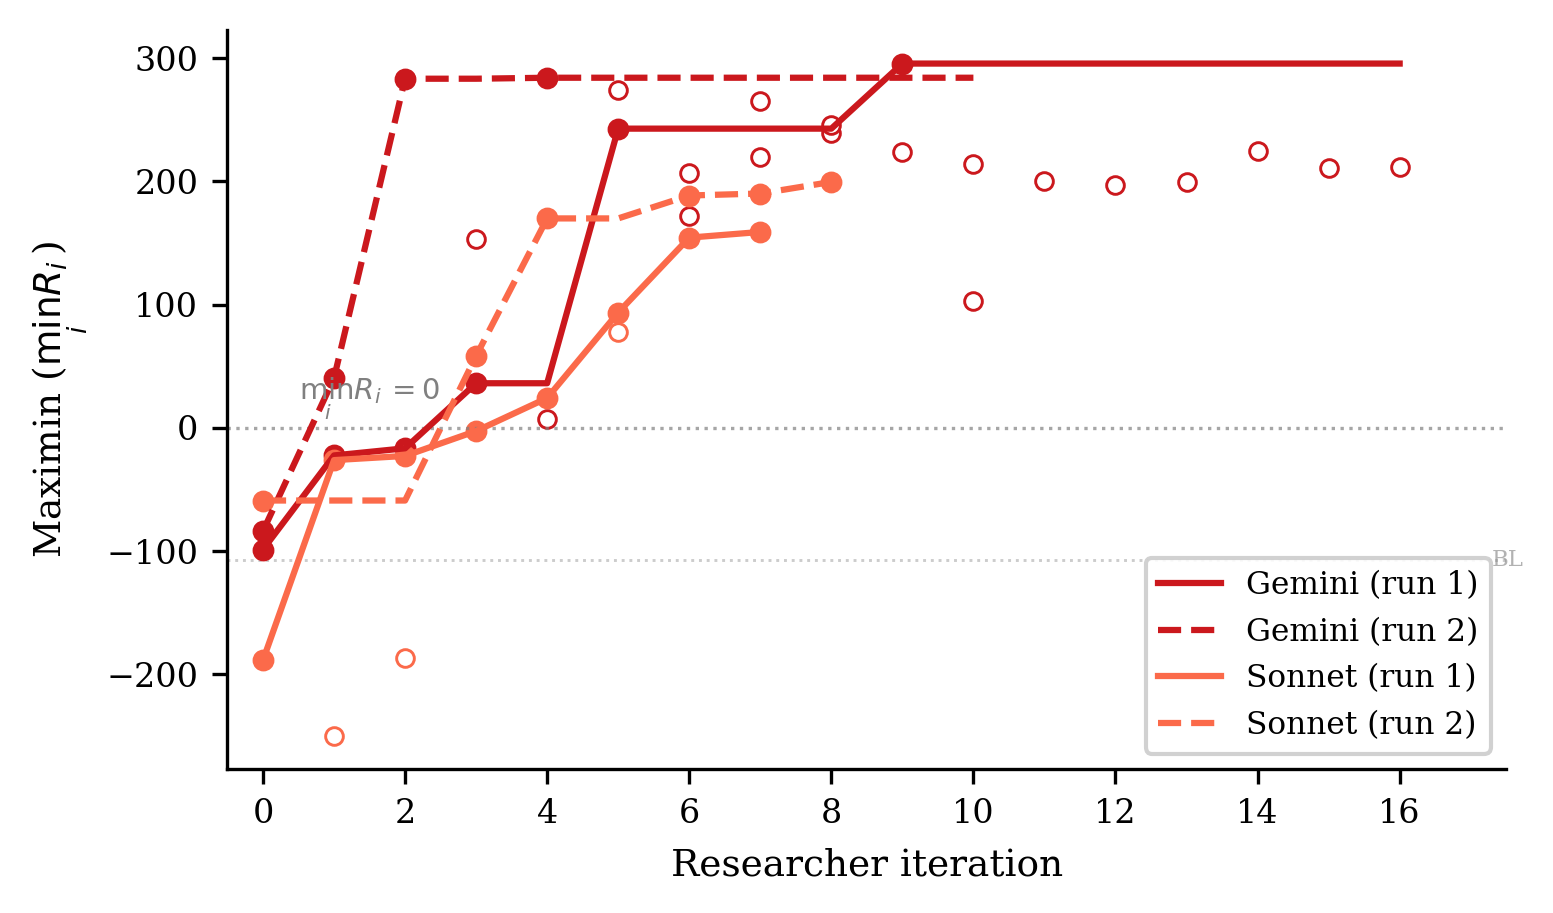
\includegraphics[width=\columnwidth]{autoresearch/figures/fig2_maximin_trajectory.png}
\caption{Maximin ($\min_i R_i$) across researcher iterations for the 4 Cleanup maximin-optimized runs. All runs transform deeply negative baselines (worst-off agents losing reward) into substantially positive values. Gemini reaches ${\sim}290$ while Sonnet reaches ${\sim}160$--$200$. The dashed line marks $\min_i R_i = 0$ (no agent loses reward overall).}
\label{fig:maximin}
\end{figure}

\begin{figure}[h]
\centering
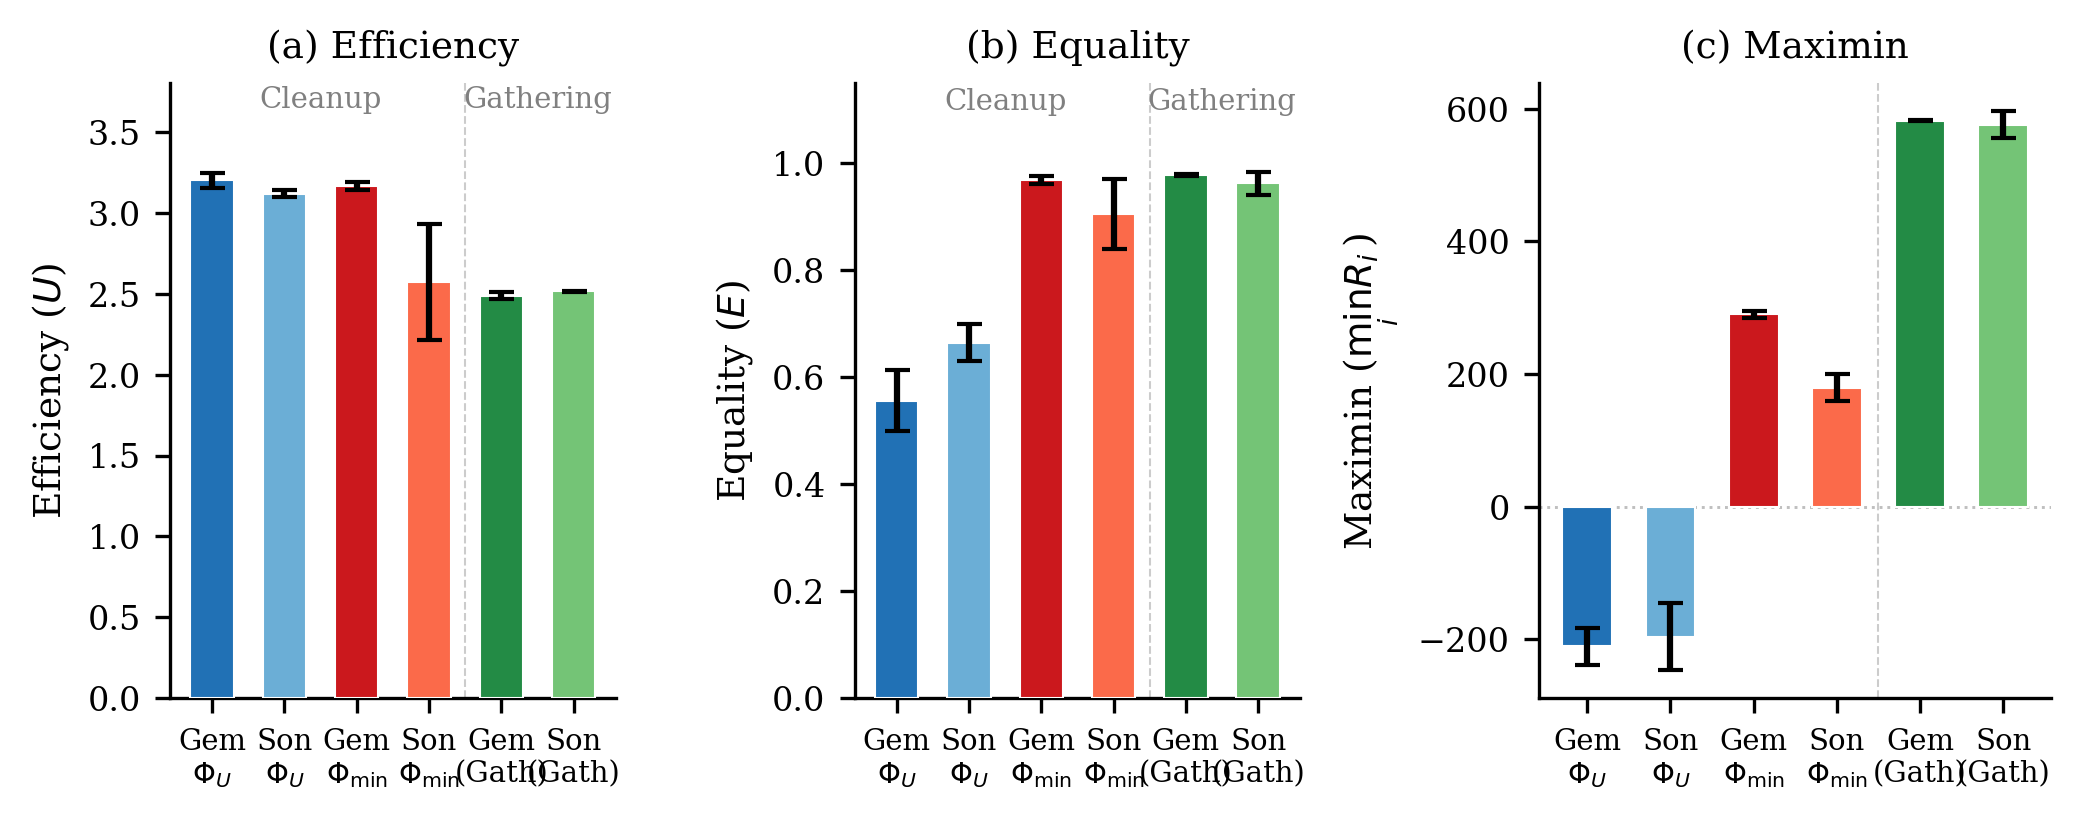
\includegraphics[width=\columnwidth]{autoresearch/figures/fig3_efficiency_equality.png}
\caption{Final efficiency ($U$, bars) and equality ($E$, hatched bars) for all 12 runs, grouped by condition. Error bars show half-range across 2 runs. Maximin-optimized Gemini runs achieve both high efficiency and near-perfect equality, while efficiency-optimized runs show moderate equality. Gathering runs achieve high equality regardless of objective.}
\label{fig:eff_eq}
\end{figure}

\end{document}
